% inspired from http://tex.stackexchange.com/questions/57152/how-to-draw-graphs-in-latex
\documentclass{article}
\thispagestyle{empty}

\usepackage{tikz}
\usetikzlibrary{positioning}
\usetikzlibrary{arrows}
\usepackage{geometry}

\geometry{hmargin=1cm, vmargin = 1cm}

\begin{document}

% Exemple de graphe pondéré positivement

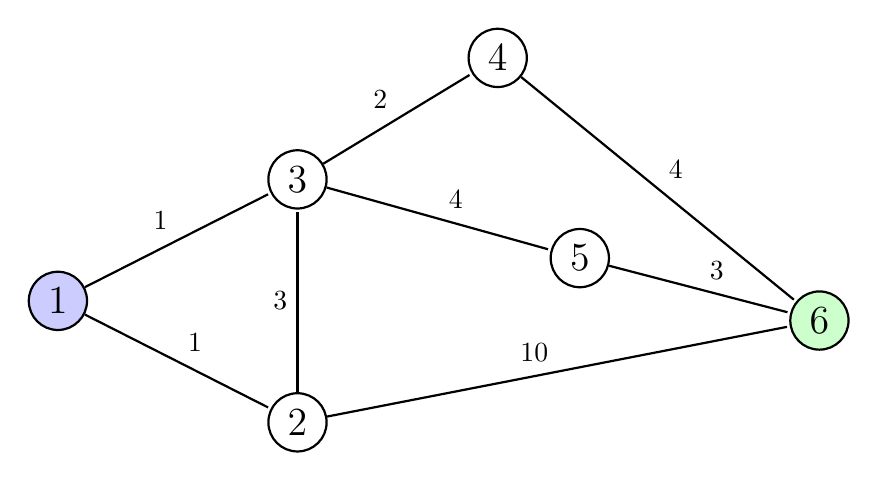
\begin{tikzpicture}[ shorten >=1pt, auto, node distance = 3cm, thick, 
   node/.style = {circle, draw,
                     font = \sffamily\Large\bfseries}]
   \node[node, fill = blue!20] (1) {$1$};
   \node[node] (2) [below right = 1cm and 2.5cm of 1]{$2$};
   \node[node] (3) [above right = 1cm and 2.5cm of 1]{$3$};
   \node[node] (4) [above right = 1cm and 2cm of 3]{$4$};
   \node[node] (5) [below right = 2cm and 0.5cm of 4]{$5$};
   \node[node, fill = green!20] (6) [below right = 0.25cm and 2.5cm of 5]{$6$};

   \path (1) edge node {$1$} (2);
   \path (1) edge node {$1$} (3);
   \path (2) edge node {$3$} (3);
   \path (2) edge node {$10$} (6);
   \path (3) edge node {$2$} (4);
   \path (3) edge node {$4$} (5);
   \path (4) edge node {$4$} (6);
   \path (5) edge node {$3$} (6);

\end{tikzpicture}

% Tour 1 :

\vspace{1cm}

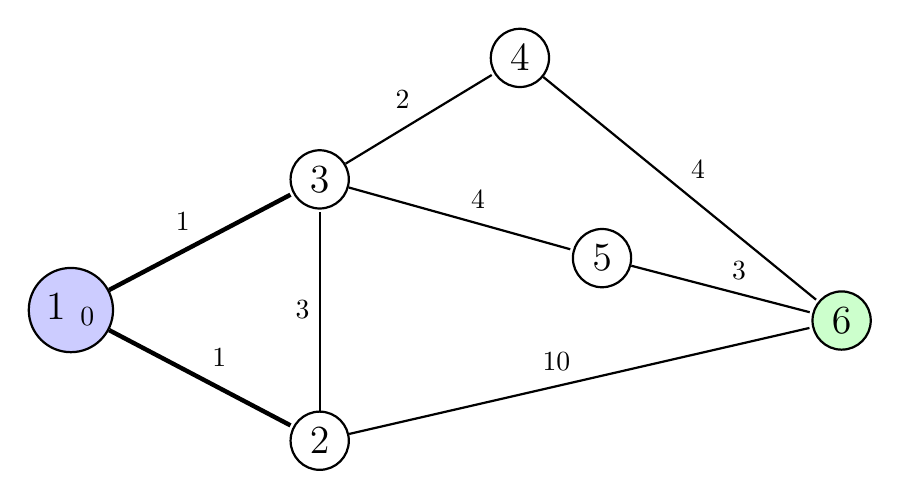
\begin{tikzpicture}[ shorten >=1pt, auto, node distance = 3cm, thick, 
   node/.style = {circle, draw,
                     font = \sffamily\Large\bfseries}]
   \node[node, fill = blue!20] (1) {$1$ $_0$};
   \node[node] (2) [below right = 1cm and 2.5cm of 1]{$2$};
   \node[node] (3) [above right = 1cm and 2.5cm of 1]{$3$};
   \node[node] (4) [above right = 1cm and 2cm of 3]{$4$};
   \node[node] (5) [below right = 2cm and 0.5cm of 4]{$5$};
   \node[node, fill = green!20] (6) [below right = 0.25cm and 2.5cm of 5]{$6$};

   \path[ultra thick] (1) edge node {$1$} (2);
   \path[ultra thick] (1) edge node {$1$} (3);
   \path (2) edge node {$3$} (3);
   \path (2) edge node {$10$} (6);
   \path (3) edge node {$2$} (4);
   \path (3) edge node {$4$} (5);
   \path (4) edge node {$4$} (6);
   \path (5) edge node {$3$} (6);

\end{tikzpicture}

% Tour 2 :

\vspace{1cm}

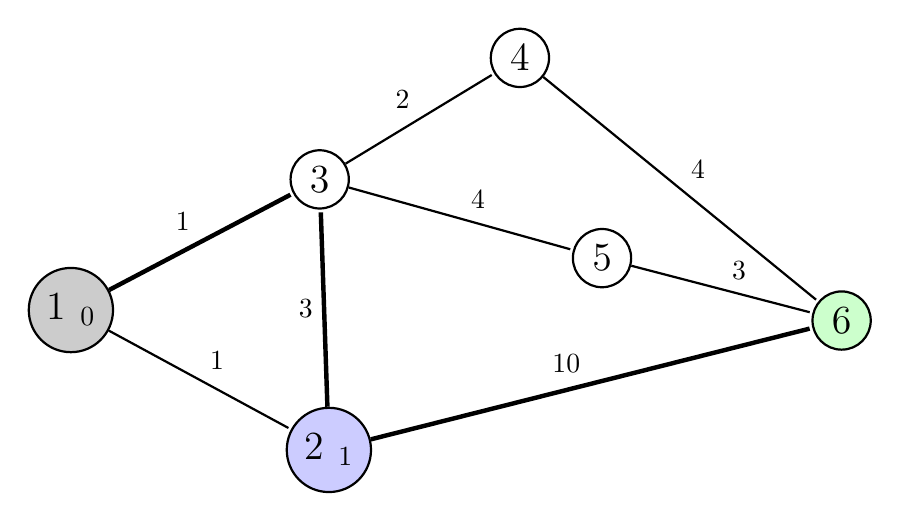
\begin{tikzpicture}[ shorten >=1pt, auto, node distance = 3cm, thick, 
   node/.style = {circle, draw,
                     font = \sffamily\Large\bfseries}]
   \node[node, fill = black!20] (1) {$1$ $_0$};
   \node[node, fill = blue!20] (2) [below right = 1cm and 2.5cm of 1]{$2$ $_1$};
   \node[node] (3) [above right = 1cm and 2.5cm of 1]{$3$};
   \node[node] (4) [above right = 1cm and 2cm of 3]{$4$};
   \node[node] (5) [below right = 2cm and 0.5cm of 4]{$5$};
   \node[node, fill = green!20] (6) [below right = 0.25cm and 2.5cm of 5]{$6$};

   \path (1) edge node {$1$} (2);
   \path [ultra thick] (1) edge node {$1$} (3);
   \path [ultra thick] (2) edge node {$3$} (3);
   \path [ultra thick] (2) edge node {$10$} (6);
   \path (3) edge node {$2$} (4);
   \path (3) edge node {$4$} (5);
   \path (4) edge node {$4$} (6);
   \path (5) edge node {$3$} (6);

\end{tikzpicture}

% Tour 3 : 

\vspace{1cm}

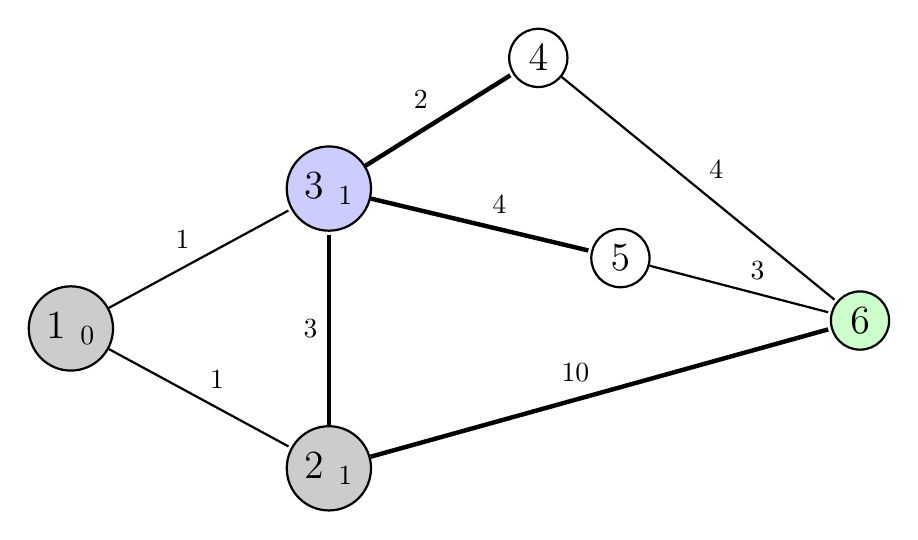
\begin{tikzpicture}[ shorten >=1pt, auto, node distance = 3cm, thick, 
   node/.style = {circle, draw,
                     font = \sffamily\Large\bfseries}]
   \node[node, fill = black!20] (1) {$1$ $_0$};
   \node[node, fill = black!20] (2) [below right = 1cm and 2.5cm of 1]{$2$ $_1$};
   \node[node, fill = blue!20] (3) [above right = 1cm and 2.5cm of 1]{$3$ $_1$};
   \node[node] (4) [above right = 1cm and 2cm of 3]{$4$};
   \node[node] (5) [below right = 2cm and 0.5cm of 4]{$5$};
   \node[node, fill = green!20] (6) [below right = 0.25cm and 2.5cm of 5]{$6$};

   \path (1) edge node {$1$} (2);
   \path (1) edge node {$1$} (3);
   \path [ultra thick] (2) edge node {$3$} (3);
   \path [ultra thick] (2) edge node {$10$} (6);
   \path [ultra thick] (3) edge node {$2$} (4);
   \path [ultra thick] (3) edge node {$4$} (5);
   \path (4) edge node {$4$} (6);
   \path (5) edge node {$3$} (6);

\end{tikzpicture}

% Tour 4 : 

\vspace{1cm}

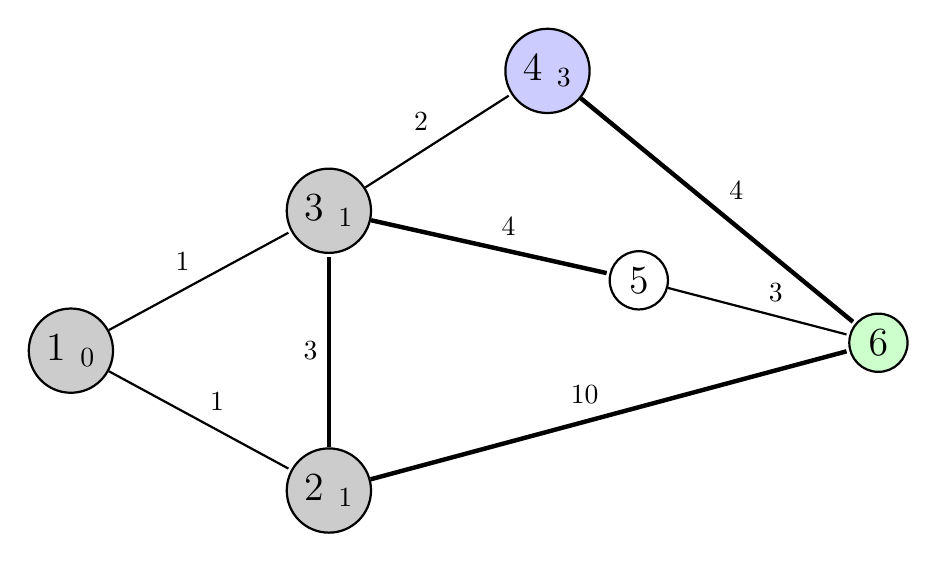
\begin{tikzpicture}[ shorten >=1pt, auto, node distance = 3cm, thick, 
   node/.style = {circle, draw,
                     font = \sffamily\Large\bfseries}]
   \node[node, fill = black!20] (1) {$1$ $_0$};
   \node[node, fill = black!20] (2) [below right = 1cm and 2.5cm of 1]{$2$ $_1$};
   \node[node, fill = black!20] (3) [above right = 1cm and 2.5cm of 1]{$3$ $_1$};
   \node[node, fill = blue!20] (4) [above right = 1cm and 2cm of 3]{$4$ $_3$};
   \node[node] (5) [below right = 2cm and 0.5cm of 4]{$5$};
   \node[node, fill = green!20] (6) [below right = 0.25cm and 2.5cm of 5]{$6$};

   \path (1) edge node {$1$} (2);
   \path (1) edge node {$1$} (3);
   \path [ultra thick] (2) edge node {$3$} (3);
   \path [ultra thick] (2) edge node {$10$} (6);
   \path (3) edge node {$2$} (4);
   \path [ultra thick] (3) edge node {$4$} (5);
   \path [ultra thick] (4) edge node {$4$} (6);
   \path (5) edge node {$3$} (6);

\end{tikzpicture}

% Tour 5 : 

\vspace{1cm}

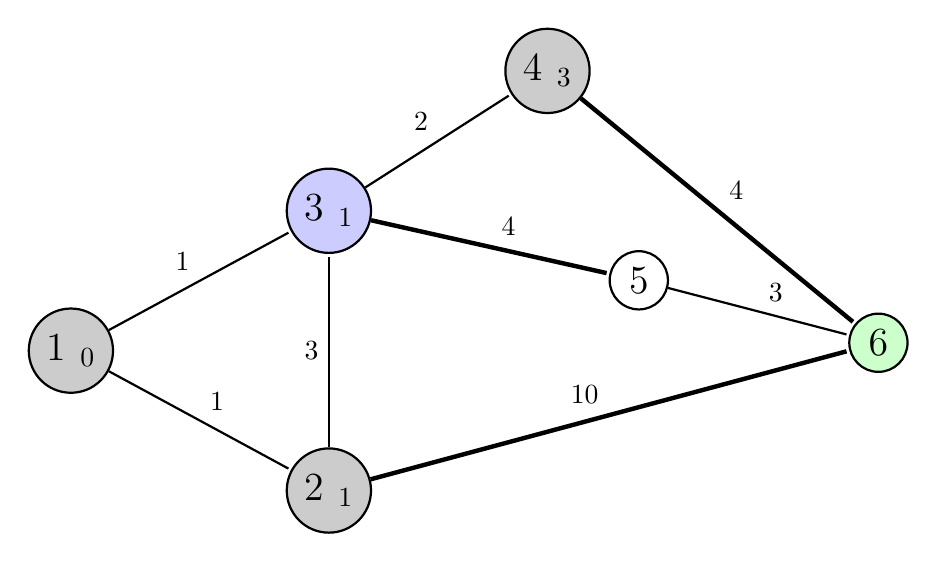
\begin{tikzpicture}[ shorten >=1pt, auto, node distance = 3cm, thick, 
   node/.style = {circle, draw,
                     font = \sffamily\Large\bfseries}]
   \node[node, fill = black!20] (1) {$1$ $_0$};
   \node[node, fill = black!20] (2) [below right = 1cm and 2.5cm of 1]{$2$ $_1$};
   \node[node, fill = blue!20] (3) [above right = 1cm and 2.5cm of 1]{$3$ $_1$};
   \node[node, fill = black!20] (4) [above right = 1cm and 2cm of 3]{$4$ $_3$};
   \node[node] (5) [below right = 2cm and 0.5cm of 4]{$5$};
   \node[node, fill = green!20] (6) [below right = 0.25cm and 2.5cm of 5]{$6$};

   \path (1) edge node {$1$} (2);
   \path (1) edge node {$1$} (3);
   \path (2) edge node {$3$} (3);
   \path [ultra thick] (2) edge node {$10$} (6);
   \path (3) edge node {$2$} (4);
   \path [ultra thick] (3) edge node {$4$} (5);
   \path [ultra thick] (4) edge node {$4$} (6);
   \path (5) edge node {$3$} (6);

\end{tikzpicture}

% Tour 6 : 

\vspace{1cm}

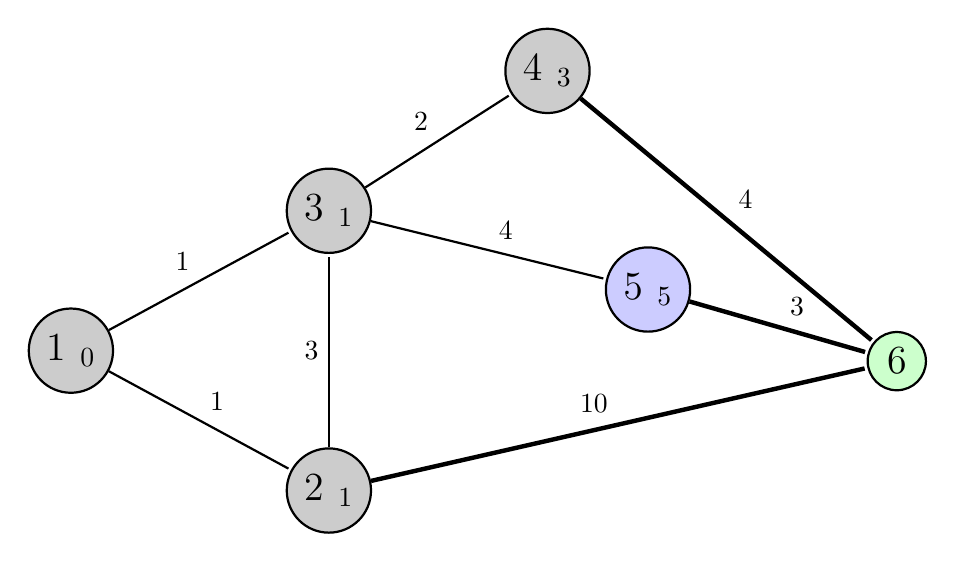
\begin{tikzpicture}[ shorten >=1pt, auto, node distance = 3cm, thick, 
   node/.style = {circle, draw,
                     font = \sffamily\Large\bfseries}]
   \node[node, fill = black!20] (1) {$1$ $_0$};
   \node[node, fill = black!20] (2) [below right = 1cm and 2.5cm of 1]{$2$ $_1$};
   \node[node, fill = black!20] (3) [above right = 1cm and 2.5cm of 1]{$3$ $_1$};
   \node[node, fill = black!20] (4) [above right = 1cm and 2cm of 3]{$4$ $_3$};
   \node[node, fill = blue!20] (5) [below right = 2cm and 0.5cm of 4]{$5$ $_5$};
   \node[node, fill = green!20] (6) [below right = 0.25cm and 2.5cm of 5]{$6$};

   \path (1) edge node {$1$} (2);
   \path (1) edge node {$1$} (3);
   \path (2) edge node {$3$} (3);
   \path [ultra thick] (2) edge node {$10$} (6);
   \path (3) edge node {$2$} (4);
   \path (3) edge node {$4$} (5);
   \path [ultra thick] (4) edge node {$4$} (6);
   \path [ultra thick] (5) edge node {$3$} (6);

\end{tikzpicture}

% Tour 7 : 

\vspace{1cm}

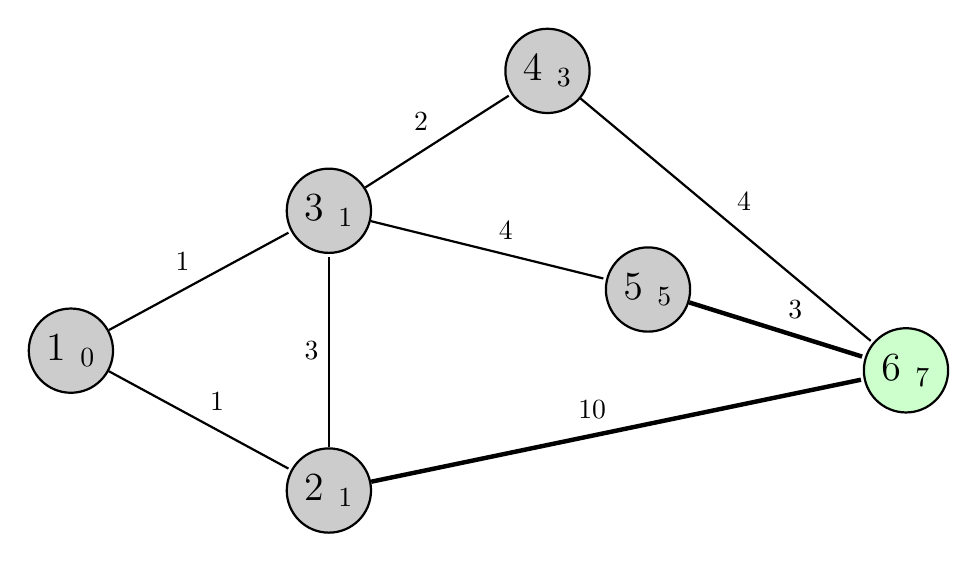
\begin{tikzpicture}[ shorten >=1pt, auto, node distance = 3cm, thick, 
   node/.style = {circle, draw,
                     font = \sffamily\Large\bfseries}]
   \node[node, fill = black!20] (1) {$1$ $_0$};
   \node[node, fill = black!20] (2) [below right = 1cm and 2.5cm of 1]{$2$ $_1$};
   \node[node, fill = black!20] (3) [above right = 1cm and 2.5cm of 1]{$3$ $_1$};
   \node[node, fill = black!20] (4) [above right = 1cm and 2cm of 3]{$4$ $_3$};
   \node[node, fill = black!20] (5) [below right = 2cm and 0.5cm of 4]{$5$ $_5$};
   \node[node, fill = green!20] (6) [below right = 0.25cm and 2.5cm of 5]{$6$ $_7$};

   \path (1) edge node {$1$} (2);
   \path (1) edge node {$1$} (3);
   \path (2) edge node {$3$} (3);
   \path [ultra thick] (2) edge node {$10$} (6);
   \path (3) edge node {$2$} (4);
   \path (3) edge node {$4$} (5);
   \path (4) edge node {$4$} (6);
   \path [ultra thick] (5) edge node {$3$} (6);

\end{tikzpicture}

% Contre-exemple : graphe pondéré négativement

\vspace{1cm}

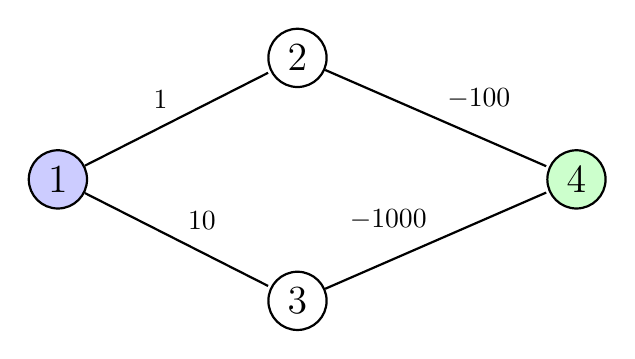
\begin{tikzpicture}[ shorten >=1pt, auto, node distance = 3cm, thick, 
   node/.style = {circle, draw,
                     font = \sffamily\Large\bfseries}]
   \node[node, fill = blue!20] (1) {$1$};
   \node[node] (2) [above right = 1cm and 2.5cm of 1]{$2$};
   \node[node] (3) [below right = 1cm and 2.5cm of 1]{$3$};
   \node[node, fill = green!20] (4) [below right = 1cm and 3cm of 2]{$4$};

   \path (1) edge node {$1$} (2);
   \path (1) edge node {$10$} (3);
   \path (2) edge node {$-100$} (4);
   \path (3) edge node {$-1000$} (4);
   
\end{tikzpicture}

% Contre-exemple 2 : ajout pour compenser les poids négatifs

\vspace{1cm}

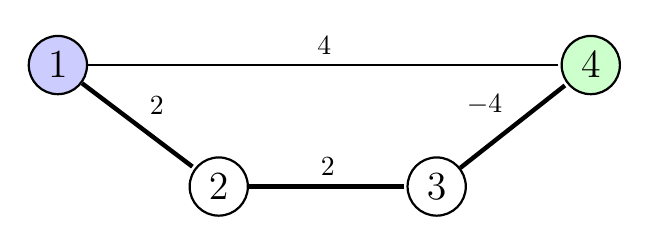
\begin{tikzpicture}[ shorten >=1pt, auto, node distance = 3cm, thick, 
   node/.style = {circle, draw,
                     font = \sffamily\Large\bfseries}]
   \node[node, fill = blue!20] (1) {$1$};
   \node[node] (2) [below right = 1cm and 1.5cm of 1]{$2$};
   \node[node] (3) [right = 2cm of 2]{$3$};
   \node[node, fill = green!20] (4) [right = 6cm of 1]{$4$};

   \path [ultra thick](1) edge node {$2$} (2);
   \path (1) edge node {$4$} (4);
   \path [ultra thick](2) edge node {$2$} (3);
   \path [ultra thick](3) edge node {$-4$} (4);
\end{tikzpicture}
\hspace{2cm}
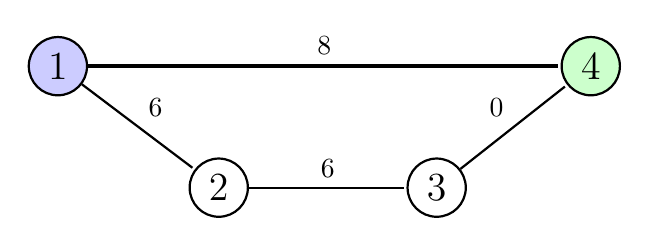
\begin{tikzpicture}[ shorten >=1pt, auto, node distance = 3cm, thick, 
   node/.style = {circle, draw,
                     font = \sffamily\Large\bfseries}]
   \node[node, fill = blue!20] (1) {$1$};
   \node[node] (2) [below right = 1cm and 1.5cm of 1]{$2$};
   \node[node] (3) [right = 2cm of 2]{$3$};
   \node[node, fill = green!20] (4) [right = 6cm of 1]{$4$};

   \path (1) edge node {$6$} (2);
   \path [ultra thick](1) edge node {$8$} (4);
   \path (2) edge node {$6$} (3);
   \path (3) edge node {$0$} (4);
\end{tikzpicture}

\end{document}
